\documentclass[11pt]{memoir}

\usepackage{vinaya-class-notes}

\title{Vinaya Class Notes}
\author{Gambhiro Bhikkhu}

\hypersetup{
  pdftitle={\thetitle},
  pdfauthor={\theauthor},
  pdfcopyright={Copyright (C) \the\year, \theauthor},
  pdfsubject={buddhism, vinaya},
  pdfkeywords={buddhism, vinaya},
  pdflicenseurl={https://creativecommons.org/licenses/by-nc-nd/4.0/},
  pdfcontacturl={https://vinaya-class.github.io/},
  pdflang={en},
}

\begin{document}

\frontmatter

\vspace*{-2cm}

{\centering%

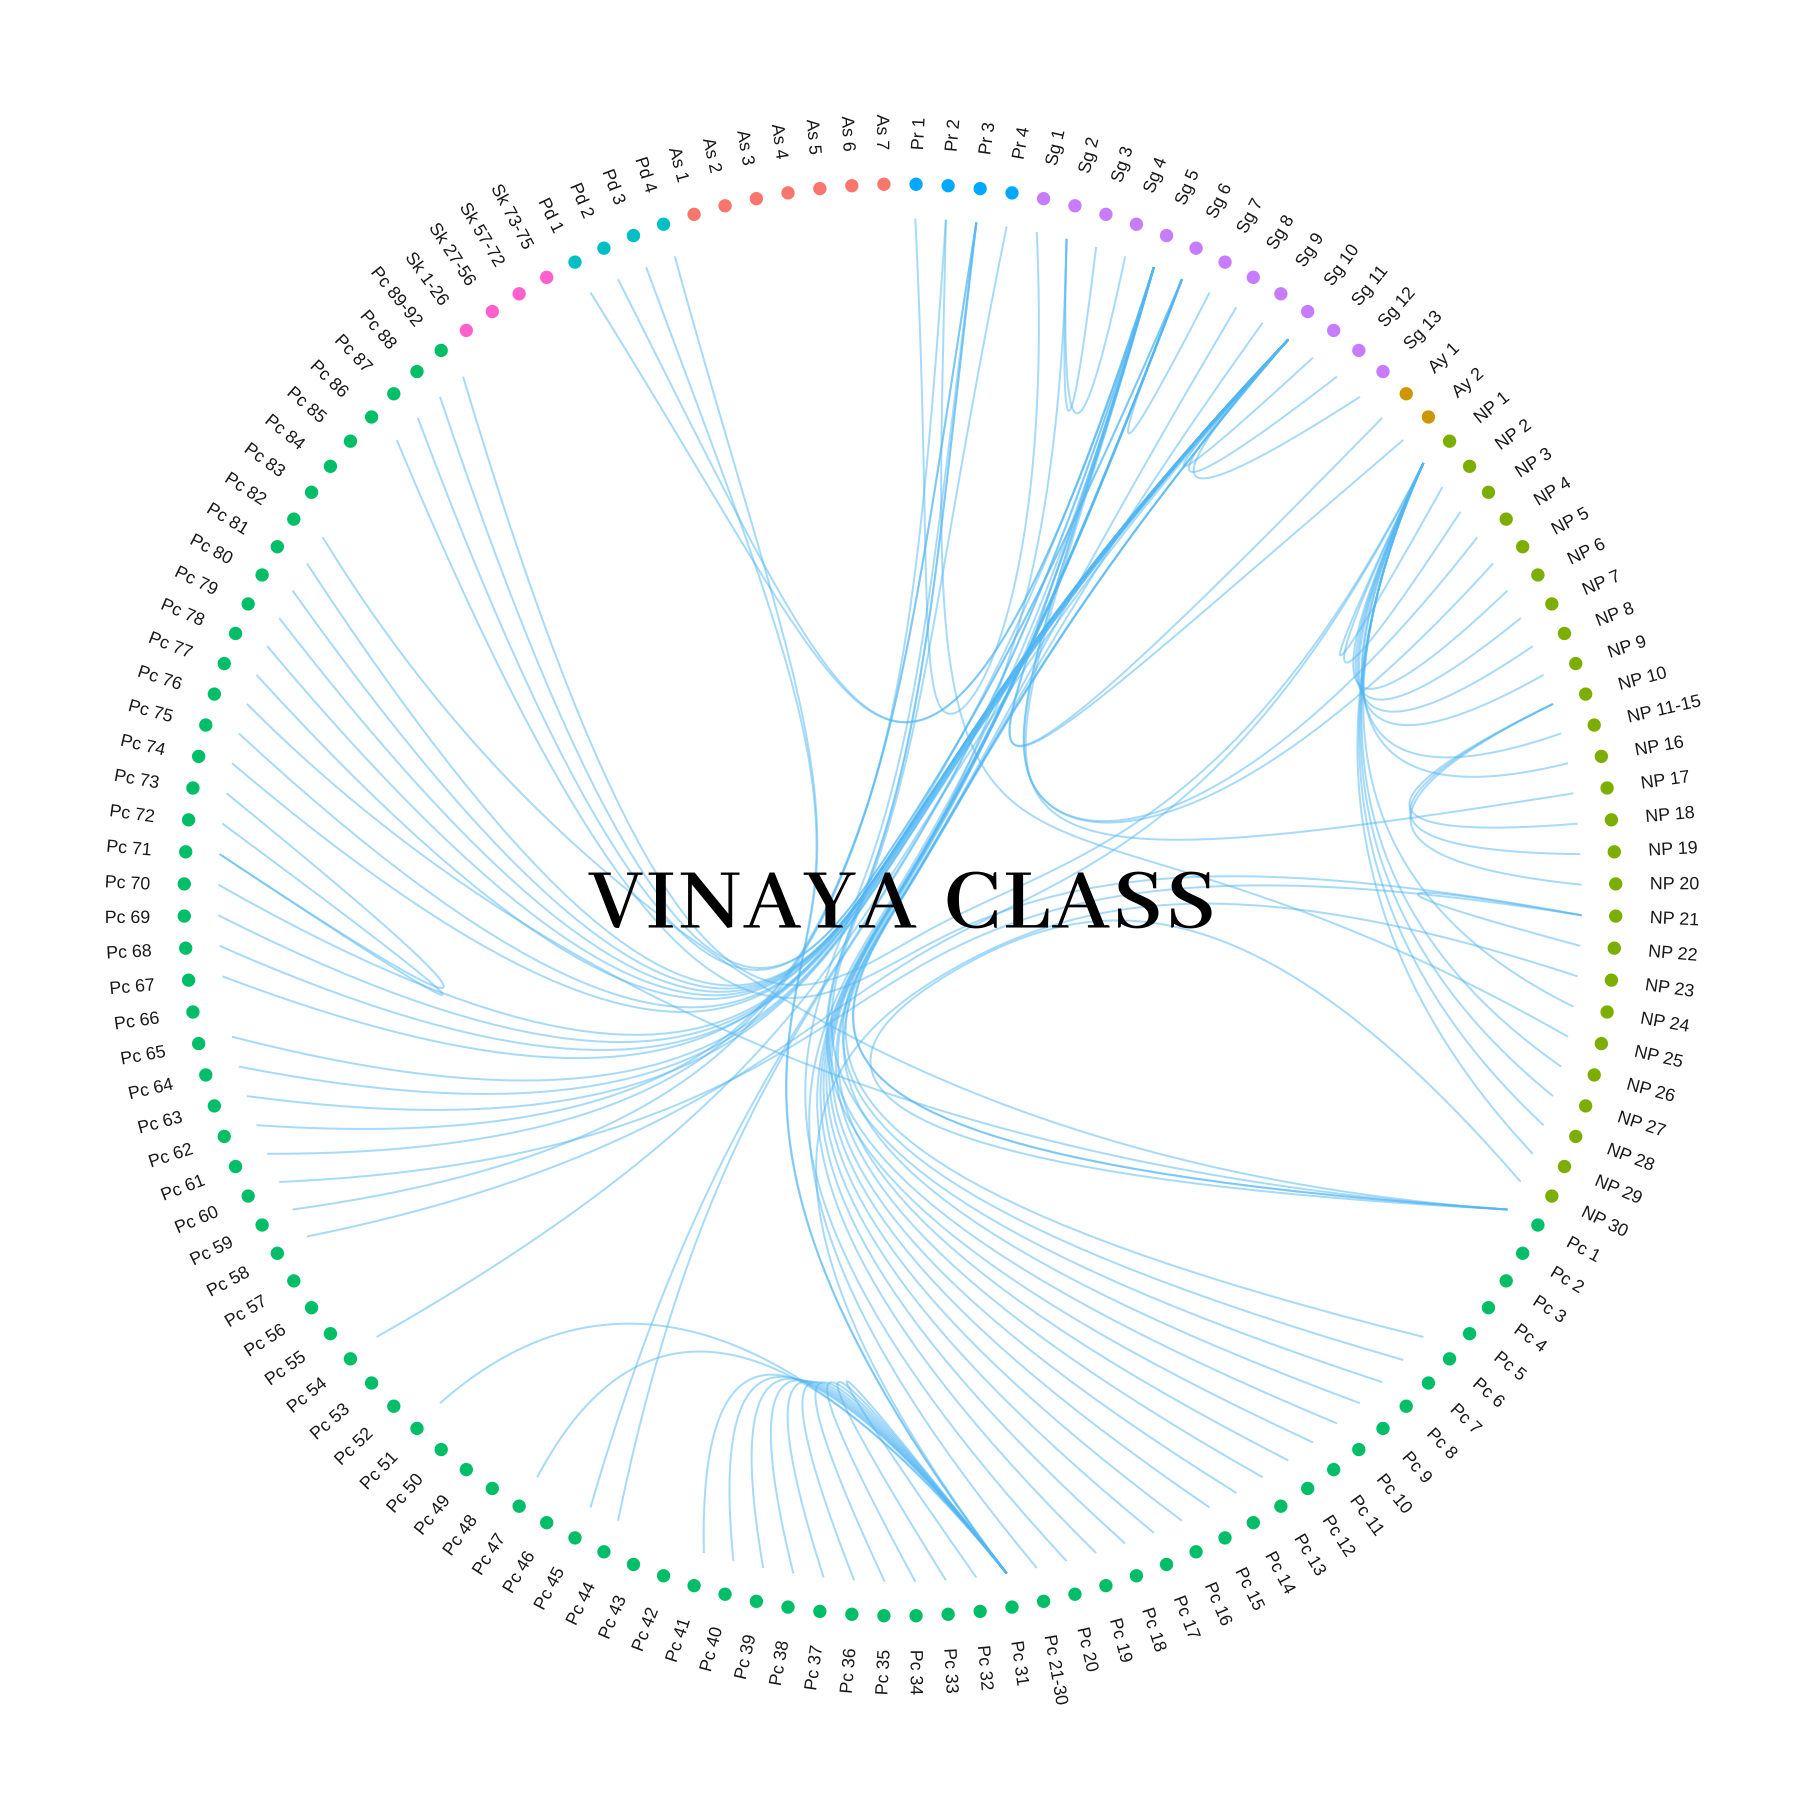
\includegraphics[width=10cm]{../../src/includes/figures/vinaya-class-title-300dpi.png}

\href{https://vinaya-class.github.io}{https://vinaya-class.github.io}

{\scshape\small last updated on}\\
\today

}

\tableofcontents*

\chapter{Introduction}
\renewcommand*{\theChapterTitle}{Introduction}

\begin{exam}{\autoExamName}

\begin{problem}

  How can a bhikkhu determine if modern items (e.g. credit cards, sun glasses) are allowable or not?

  \bigskip

  \begin{answers}{1}
    \bChoices
    \Ans0 Discuss with the community and create a new rule\eAns
    \Ans0 Follow local cultural examples\eAns
    \Ans1 Discuss and follow the Four Great Standards\eAns
    \Ans0 One cannot know for sure what the Buddha's intentions were\eAns
    \eChoices
  \end{answers}

  \begin{solution}
    Suitable protocol for a community to discuss how to apply the Four Great
    Standards and agree on the accepted standards.
  \end{solution}

\end{problem}

\problemDivide

\begin{problem}

  A bhikkhu is visiting a friend who asks if it's all right for them to eat a
  pizza in the evening. The bhikkhu says it's fine by him, and they eat the pizza.
  \emph{Is this an offence?}

  \bigskip

  \begin{answers}{1}
    \bChoices
    \Ans0 No, because they are not in the monastery\eAns
    \Ans0 No, but there is a partial offence\eAns
    \Ans0 Usually it is, but it can depend on the situation\eAns
    \Ans1 Yes, it is a pācittiya offence\eAns
    \eChoices
  \end{answers}

  \bigskip

  \textbf{Discussion:} How does one determine whether there is full offence of a
  rule? What happens when not all factors are fulfilled for an offence?

  \begin{solution}
    Consider which of the five factors are fulfiled in the situation.
  \end{solution}

\end{problem}

\problemDivide

\begin{problem*}

  Match the type of offence with its description.

  \bigskip

  \begin{multicols}{2}

    \begin{parts}

    \item \fillin{2cm}{\ref{parajika}} pārājika
    \item \fillin{2cm}{\ref{sanghadisesa}} saṅghādisesa
    \item \fillin{2cm}{\ref{thullacaya}} thullacāya
    \item \fillin{2cm}{\ref{pacittiya}} pācittiya
    \item \fillin{2cm}{\ref{nissaggiya}} nissaggiya pācittiya
    \item \fillin{2cm}{\ref{dukkata}} dukkaṭa

    \columnbreak

    \bMatchChoices

    \item\label{thullacaya} grave offence
    \item\label{parajika} defeat
    \item\label{pacittiya} offence to be confessed
    \item\label{dukkata} wrong-doing
    \item\label{nissaggiya} involving forfeiture
    \item\label{sanghadisesa} involving community meetings

    \eMatchChoices
      
    \end{parts}
    
  \end{multicols}

  \bigskip

  \textbf{Discussion:} Advice on restoring one's faith after breaking a rule or
  having done something regrettable.

  \begin{solution}
    The classes of offences are: (1) pārājika, (2) saṅghādisesa, (3) thullacāya,
    (4) pācittiya, (5) nissaggiya pācittiya, (6) dukkaṭa.
  \end{solution}

\end{problem*}

\problemDivide

\begin{problem*}

  \begin{parts}

  \item Ignoring a \emph{sekhiya} etiquette rule out of disrespect for the
    training is\ldots

    \begin{answers}{4}
      \bChoices
      \Ans1 a wrong-doing\eAns
      \Ans0 to be confessed\eAns
      \Ans0 involves community meetings\eAns
      \Ans0 negligible, \emph{abbohārika}\eAns
      \eChoices
    \end{answers}

  \item Probation is a procedure following a \ldots{} offence.

    \begin{answers}{4}
      \bChoices
      \Ans0 pārājika\eAns
      \Ans1 saṅghādisesa\eAns
      \Ans0 pācittiya\eAns
      \Ans0 dukkaṭa\eAns
      \eChoices
    \end{answers}

  \end{parts}
  
  \bigskip

  \begin{solution}
    Mānatta is the penance, parivāsa is the probation procedure following a saṅghādisesa offence.
  \end{solution}

\end{problem*}

%\clearpage

\begin{problem*}

  \textbf{True} or \textbf{False}.

  \bigskip

  \begin{parts}

  \item \TF{F} Breaking a rule is always an offence for a bhikkhu, even if he doesn't
    remember the rule.

    \bigskip

    \textbf{Discussion:} Consider the case when he remembers, but goes ahead because the job has to be finished today.
    What is the proper protocol for him to follow?

  \item \TF{F} One of the Four Great Standards is that if it is not already allowed,
    but doesn't follow what is desirable, then it is allowable.

  \item \TF{F} During his upasampada, the candidate chants several lines of the
    ceremony incorrectly, therefore his ordination is invalid.

    \bigskip

    \textbf{Discussion:} What is essential for a valid bhikkhu upasampada?
    
  \item \TF{F} A young man (over 20) receives upasampada. He has concealed that
    he has to pay back his student loan, therefore his ordination is invalid.

  \item \TF{F} A bhikkhu's \emph{mentor} and \emph{preceptor} cannot be the same
    person.

  \item \TF{F} A bhikkhu complains about the monastic life and says, `Who am I kidding? Really,
    I want to disrobe.' After this statement he is no longer a bhikkhu.

    \bigskip

    \textbf{Discussion:} What are the factors of the disrobing procedure?

  \item \TF{F} A bhikkhu can request a \emph{baisuddhi} document when he arrives in Thailand.

    \bigskip

    \textbf{Discussion:} What is a \emph{baisuddhi}, who issues it, and what happens if you don't have one in Thailand?

  \item \TF{T} The community may decide to give a bhikkhu a new robe from the stores without formal \emph{sanghakamma}. 

    \bigskip

    \textbf{Discussion:} What are the steps of formal \emph{sanghakamma}?

  \end{parts}

\end{problem*}

\problemDivide

\begin{problem}

  The abbot of a monastery tells the community that in this monastery, the
  standard is that the last person finishing the meal must always empty the
  water from the spittoons and put away the seats. One monk, being in a hurry,
  doesn't do so and mosquitoes start breeding in the spittoon water. Are there
  offences?

  \bigskip

  \begin{answers}{4}
    \bChoices
    \Ans0 pārājika\eAns
    \Ans1 pācittiya\eAns
    \Ans0 dukkaṭa\eAns
    \Ans0 no offences\eAns
    \eChoices
  \end{answers}

\end{problem}

\bigskip

\textbf{Discussion:} What are some examples of local standards, or \emph{korwat}
rules? Cf. MN 48, Uda 4.5, Mv X on disputes at Kosambī. The Buddha then visits
the park where Ven. Anuruddha, Nandiya and Kimbila were living in harmony,
blending as `milk and water' (MN 31).

\problemDivide

\begin{problem}

  A bhikkhu lives alone in an accomodation on the property of his supporters. Some of
  his visitors consider him very accomplished and wish to join the monastic practice.
  What are the type of ordinations he can he give them?

  \bigskip

  \begin{manswers}{4}
    \bChoices
    \Ans0 bhikkhu\eAns
    \Ans1 samanera\eAns
    \Ans1 anagārika\eAns
    \Ans0 being alone, he can't ordain them\eAns
    \eChoices
  \end{manswers}

\end{problem}

\bigskip

\textbf{Discussion:} Who can act as a preceptor \emph{upajjhāya} to ordain bhikkhus?

\end{exam}



\mainmatter

\chapter{Killing and Harming}

\begin{itemize}
\tightlist
\item
  \textbf{Pr 3,} Killing a human being
\item
  \textbf{Pc 61,} Killing an animal
\item
  \textbf{Pc 20,} Pouring water containing living beings
\item
  \textbf{Pc 62,} Drinking water containing living beings
\item
  \textbf{Pc 10,} Digging soil
\item
  \textbf{Pc 11,} Damaging living plants or seeds
\end{itemize}

\section{Pr 3, Killing a human being}

\includemap{../../src/includes/mindmaps/pr-3.png}

\textbf{Origin:} bhikkhus develop aversion to the body and kill
themselves or ask an assassin to kill them.

Recommending death or euthanasia can be \textbf{parajika} if the
instruction is followed. Hinting fulfils effort, such as ``death would
be better for you''.

A human being is regarded as such from the time when the `being to be
born' is established in the womb. This is an uncertain time, sometime
after conception during embryo development. The embryo can't develop
otherwise.

\clearpage

\begin{quote}
``If consciousness were not to descend into the mother's womb, would
name-and-form take shape in the womb?''

``No, lord.''

``If, after descending into the womb, consciousness were to depart,
would name-and-form be produced for this world?''

``No, lord.''

``If the consciousness of the young boy or girl were to be cut off,
would name-and-form ripen, grow, and reach maturity?''

``No, lord.''

(\href{https://www.accesstoinsight.org/tipitaka/dn/dn.15.0.than.html}{DN
15})
\end{quote}

\section{Pc 61, Killing an animal}

Giving an order fulfils effort.

\textbf{Result} is a factor.

Doesn't include animals smaller than visible to the naked eye. Doesn't
include accidents (sweeping). No room for `phrasing it right'.

Origin: Ven. Udayin is killing crows by shooting them with arrows,
cutting their heads off and putting them in a row on a stake. The Buddha
scolds him, ``How can you, foolish man, intentionally deprive a living
thing of life? \ldots{}''
(\href{https://suttacentral.net/pli-tv-bu-vb-pc61/en/horner}{Vibh. Pc
61})

Mercy killing by the owner, or euthanasia practices by vets fulfil
effort. Having a pet means responsibility.

Acting in doubt, going ahead anyway is dukkata. Such as when the bhikkhu
thinks that cleaning an item may or may not kill living beings. Trying
carefully not to kill insects while cleaning is not an offence.

\textbf{Perception} is a factor. Stepping on a twig with the intention
to crush a snake is dukkata.

\section{Pc 20, Pouring water containing living beings}

Knowing they will die from pouring it. It can also include knowingly
adding poisonous substances.

If the water doesn't contain living beings, but the bhikkhu thinks it
does, pouring or using it is dukkata.

Giving an order fulfils effort.

Result is not a factor. Doesn't include accidents.

Can't water plants if one plans to eat its fruit, but may indicate it
for others.

Kutis may use small gutters as water moats around the stilts to keep out
ants. One has to treat the water with household chemicals, otherwise
mosquitoes will breed in the water.

\section{Pc 62, Drinking water containing living beings}

\enlargethispage{\baselineskip}

Knowing they will die from drinking it, even accidentally.

Using water strainers or robe. Determining a corner of the sanghati as a
water-filter.

Result is not a factor.

\clearpage

\section{Pc 10, Digging soil}

\begin{multicols}{2}

\textbf{Origin:} relates to the ancient belief that soil is alive, and
loses life when dug up.

\textbf{Object:} `genuine' soil.

\emph{Not} genuine soil:

\begin{itemize}
\tightlist
\item
  dust from wind erosion
\item
  pure or mostly rock, stones, gravel, sand are never `genuine' soil
\item
  burnt or already dup up soil is not `genuine' until rained on for four
  months
\end{itemize}

If someone digs up the soil, a bhikkhu may shovel it into a wheelbarrow
without offence.

\textbf{Effort:} Digging, burning, making a hole, or giving command to
do it.

Putting tent pegs in the ground is to be confessed.

\columnbreak

\textbf{Non-offenses:}

\begin{itemize}
\tightlist
\item
  unknowingly, unthinkingly, unintentionally
\item
  indicating a general need or task
\item
  asking for clay or or soil
\item
  digging a trapped person or animal out
\end{itemize}

Allowance to indicate a need or general task to a lay person by
``wording it right (\emph{kappiya-vohāra},''allowable expression," or
``wording it right'').

A specific command would be an offense (`dig a hole here'), but an
indication (`dig a hole') of a desire or intent would not (`it would be
good to have a hole for this post').

\end{multicols}

\section{Pc 11, Damaging living plants or seeds}

\begin{multicols}{2}

\textbf{Origin:} a bhikkhu cuts down a tree where a deva was living. The
rule is formed later, when people complained of the bhikkhus mistreating
one-facultied life.

\textbf{Object:} Living plant or seed. Lower plant life (i.e.~mold,
algae, fungi) is not included.

\textbf{Effort:} cutting, breaking, cooking, or getting others to do it.

\textbf{Fruit with seeds:} allowance to make allowable (kappiyam). Fruit
can be kappied in one ``heap''.

\columnbreak

To `kappi' fruit is about the feelings of the donor, not killing the
fruit or transfering kamma.

Knowingly eating un-kappied seeds is dukkata.

\textbf{Non-offenses:}

\begin{itemize}
\tightlist
\item
  unknowingly, unthinkingly, unintentionally
\item
  asking a lay person for flowers etc. in general, or indicating a
  general task
\item
  removing branches or leaves which are already dead
\item
  can cut a trapped person or animal out
\item
  counter-fire
\end{itemize}

\end{multicols}
\par
\enlargethispage{2\baselineskip}

\textbf{Note:} Pc 10 and Pc 11 prevents bhikkhus from engaging in
agriculture, which is probably part of the intended results, although
not their direct origin.


\chapter{2. Stealing}
\renewcommand*{\theChapterTitle}{2. Stealing}

\begin{exam}{\autoExamName}

\begin{problem*}

  Are there offences?

\begin{parts}

  \item A bhikkhu sneaks into the kitchen and eats an apple.

  \bigskip

  \begin{answers}{5}
    \bChoices
    \Ans0 pārājika\eAns
    \Ans0 thullacāya\eAns
    \Ans1 pācittiya\eAns
    \Ans0 dukkaṭa\eAns
    \Ans0 no offences\eAns
    \eChoices
  \end{answers}

  \bigskip

  \begin{solution}
    Pācittiya for eating unoffered food, another pacittiya if eating in the
    wrong time. Stealing doesn't apply if the contents of the kitchen are
    considered Sangha property.
  \end{solution}

  \item The same bhikkhu sees a wallet left on the kitchen counter and picks it
    up, hoping to find money in it. He only finds ID cards, so he takes the wallet
    to the monk's office for safe-keeping.

  \bigskip

  \begin{answers}{5}
    \bChoices
    \Ans0 pārājika\eAns
    \Ans1 thullacāya\eAns
    \Ans0 pācittiya\eAns
    \Ans0 dukkaṭa\eAns
    \Ans0 no offences\eAns
    \eChoices
  \end{answers}

  \begin{solution}
    Stealing is complete as soon as picking it up. Thullacāya, because there are
    no valuables.
  \end{solution}

  \bigskip

  \item A man gives a bhikkhu a new phone as a gift. He says he was able to get it very cheaply.
  The bhikkhu doesn't know that the phone comes from a batch stolen from the factory. 

  \bigskip

  \begin{answers}{5}
    \bChoices
    \Ans0 pārājika\eAns
    \Ans0 thullacāya\eAns
    \Ans0 pācittiya\eAns
    \Ans0 dukkaṭa\eAns
    \Ans1 no offences\eAns
    \eChoices
  \end{answers}

  \begin{solution}
    There is no offense assigned for receiving stolen goods, even knowingly.
  \end{solution}

  \bigskip

  \item A bhikkhu is visiting a monastery. He is frustrated that he is not given
    the WiFi password. He uses a program on his laptop to break the WiFi encryption
    and steal the password anyway.

  \bigskip

  \begin{answers}{5}
    \bChoices
    \Ans0 pārājika\eAns
    \Ans0 thullacāya\eAns
    \Ans0 pācittiya\eAns
    \Ans1 dukkaṭa\eAns
    \Ans0 no offences\eAns
    \eChoices
  \end{answers}

  \begin{solution}
    Dukkaṭa for a broken promise. `Stealing a password' is colloquial language
    for `copying without permission'.
  \end{solution}

  \bigskip

  \textbf{Discussion:} What if this is in a hotel where they charge for WiFi access?

  \begin{solution}
    Dukkaṭa for a broken promise, pacittiya if deceit is involved. Using services without permission is not stealing.
  \end{solution}

  \bigskip

  \item A bhikkhu is preparing to visit England. A visitor at the monastery asks
    him to carry an expensive audio recorder with him and give it to his friend in
    England. The bhikkhu decides to keep the recorder.

  \bigskip

  \begin{answers}{5}
    \bChoices
    \Ans0 pārājika\eAns
    \Ans0 thullacāya\eAns
    \Ans0 pācittiya\eAns
    \Ans1 dukkaṭa\eAns
    \Ans0 no offences\eAns
    \eChoices
  \end{answers}

  \begin{solution}
    Parajika if the recorder is seen as the friend's property.
    Dukkaṭa for a broken promise.

    Make sure to clarify intentions, ask again for
    clear statements if necessary.

    `I give this to you, please give it to X' -- he is given ownership of the
    item, and \emph{promises} to give it to X.

    `This is my friend's recorder, please take it to him' -- he is not given
    ownership, if he keeps it, the penalty is parajika.
  \end{solution}

  \bigskip

  \item A bhikkhu receives a bag of expensive sweets on alms-round from a lady, who
  says, `I bought these for the abbot'. The bhikkhu eats a bit from it before giving it
  to the abbot.

  \bigskip

  \begin{answers}{5}
    \bChoices
    \Ans0 pārājika\eAns
    \Ans1 thullacāya\eAns
    \Ans0 pācittiya\eAns
    \Ans1 dukkaṭa\eAns
    \Ans0 no offences\eAns
    \eChoices
  \end{answers}

  \begin{solution}
    Thullacāya because he only eats a small bit, not the whole bag. Dukkaṭa for a broken promise.
  \end{solution}

  \bigskip

  \item A senior bhikkhu places a bowl under shared ownership (\emph{vikappana}) with a samanera.
  He tells the bhikkhu that he may take it anytime when he needs it, and keeps the bowl in his kuti.
  A year later, the samanera is now a junior bhikkhu.
  The senior bhikkhu takes the bowl from the kuti when the junior bhikkhu is not there.

  \bigskip

  \begin{answers}{5}
    \bChoices
    \Ans0 pārājika\eAns
    \Ans0 thullacāya\eAns
    \Ans0 pācittiya\eAns
    \Ans0 dukkaṭa\eAns
    \Ans1 no offences\eAns
    \eChoices
  \end{answers}

  \begin{solution}
    No offense for taking items on trust when there has been a previous
    arrangement. In this case, no offense for using a \textit{vikappana} item:
    the \emph{vikappana} is automatically rescinded when items are taken on
    trust.
  \end{solution}

  \item A bhikkhu is visiting a monastery and makes a long phone call. The call
  costs €100. The resident monks discover it on the bill and ask if
  anyone knows about this call. He remains silent.

  \bigskip

  \begin{answers}{5}
    \bChoices
    \Ans0 pārājika\eAns
    \Ans0 thullacāya\eAns
    \Ans1 pācittiya\eAns
    \Ans1 dukkaṭa\eAns
    \Ans0 no offences\eAns
    \eChoices
  \end{answers}

  \begin{solution}
    Dukkaṭa for the broken promise (using unauthorized services). Pācittiya for deceit.
  \end{solution}

\end{parts}

\end{problem*}

\end{exam}

\section*{Discussion}

How is it possible for a bhikkhu to steal from the Sangha?

\bigskip

A bhikkhu drives away with the monastery car and never comes back.
What are the consequences?


\chapter{3. Sexual Conduct}
\renewcommand*{\theChapterTitle}{3. Sexual Conduct}

\begin{exam}{\autoExamName}

\begin{problem}

  A bhikkhu is staying at the apartment of a friend, where they organize a small
  gathering, and they start drinking alcohol. The bhikkhu gets drunk, and
  eventually he goes to bed in his room. He wakes up, and finds a woman's
  underwear in his bed, with a note saying `love and kisses', plus a used
  condom.

  Is the bhikkhu pārājika? 

  \bigskip
 
  \begin{answers}{1}
    \bChoices
    \Ans0 No, because he was drunk\eAns
    \Ans0 No, if he was practising trantric freedom and compassion\eAns
    \Ans1 Yes, since there is clear evidence of intercourse\eAns
    \Ans0 Yes, even if he can't remember anything\eAns
    \eChoices
  \end{answers}

  \bigskip

  \textbf{Discussion:} What if he convinces himself that he is pārājika, but
  later finds out that they had played a prank on him?
  
\end{problem}

\problemDivide

\begin{problem}

  Mark the factors which, under \textit{Sg 1}, commit a \textit{thullacāya} offence.

  \begin{answers}{6}
    \bChoices
    \Ans0 object\eAns
    \Ans0 perception\eAns
    \Ans1 intention\eAns
    \Ans1 effort\eAns
    \Ans0 result\eAns
    \eChoices
  \end{answers}

  \bigskip

  \textbf{Discussion:} describe such a situation.

\end{problem}

\problemDivide

\begin{problem*}

  Are there offences?

\begin{parts}

\item
  A women asks to speak with a bhikkhu.
  It is a hot day and she is dressed quite openly.
  For the rest of the day, he continues fantasising about her.

  \bigskip

  \begin{answers}{6}
    \bChoices
    \Ans0 pārājika\eAns
    \Ans0 saṅghādisesa\eAns
    \Ans0 thullacāya\eAns
    \Ans0 pācittiya\eAns
    \Ans0 dukkaṭa\eAns
    \Ans1 no offences\eAns
    \eChoices
  \end{answers}

  \bigskip

  \item Later, the bhikkhu recollects the meeting, starts rubbing himself, and causes an emission.

  \bigskip

  \begin{answers}{6}
    \bChoices
    \Ans0 pārājika\eAns
    \Ans1 saṅghādisesa\eAns
    \Ans0 thullacāya\eAns
    \Ans0 pācittiya\eAns
    \Ans0 dukkaṭa\eAns
    \Ans0 no offences\eAns
    \eChoices
  \end{answers}

  \bigskip

  \textbf{Discussion:} asking women to cover themselves when they come to a
  meeting in what is a normal dress for them.

  \bigskip

\end{parts}

\end{problem*}

\end{exam}

\chapter{Lustful Conduct}

\begin{itemize}
\tightlist
\item
  \textbf{Sg 2,} Lustful contact with a woman
\item
  \textbf{Sg 3,} Speaking lewd words to a woman
\item
  \textbf{Sg 4,} Praising sexual intercourse as gift
\item
  \textbf{Pc 7,} Teaching more than six sentences
\end{itemize}

\section{Sg 2, Lustful contact with a woman}

\begin{multicols}{2}

Origin: Ven. Udayin disturbing a bhrahmin's wife while they are visiting
him.

\textbf{Object:} a living woman, ``even one born on that day.'' Body,
hand, limbs, a lock of hair, etc.

\textbf{Perception:} perceiving her to be a woman.

\textbf{Intention:} impelled by lust, any state of passion, desire to
enjoy the contact. Can be an extended period of desire, or a momentary
attraction.

Contact out of filial affection for family members is a dukkata.

\textbf{Effort:} physical contact.

Items she is wearing are direct contact.

Indirect contact:

\begin{itemize}
\tightlist
\item
  touching a item which she is holding: thullacaya
\item
  touching her with an item one is holding: thullacaya
\item
  item to item: dukkata
\item
  tossing: dukkata
\item
  shaking sth. she is standing on: dukkata
\end{itemize}

Passive contact:

Contact while trying to shake her off is not an offense.

If the bhikkhu's aim is to partake, the offense is sanghadisesa.

\subsection{Non-offenses}

\begin{itemize}
\tightlist
\item
  unintentionally
\item
  unthinkingly
\item
  unknowingly
\item
  the bhikkhu doesn't give his consent
\item
  no desire for the contact
\item
  has desire, but makes no effort
\end{itemize}

\end{multicols}

\section{Sg 3, Speaking lewd words to a woman}

\begin{multicols}{2}

Wanting to enjoy saying something lewd. Directly referencing \emph{her}
genitals, anus, or her performing sexual intercourse. Slang, euphemisms,
non-verbal gestures fulfill effort.

\textbf{Object:} Any woman who recognizes lewd comments.

May not know: too young, too innocent or retarded, or doesn't know the
language.

\textbf{Perception:} The bhikkhu perceives her to be a woman.

\textbf{Intention:} Impelled by lust. The minimum lust is wanting to
enjoy saying something lewd.

\begin{itemize}
\tightlist
\item
  not necessary to have desire to have sex with her
\item
  statements in anger come under Pc 2 instead
\end{itemize}

\textbf{Effort:} Praising, criticizing, asking, etc. referencing her
genitals, anus, or her performing sexual intercourse.

\begin{itemize}
\tightlist
\item
  direct mention of above
\item
  indirect references, slang, euphemisms, non-verbal gestures fulfill
  effort
\end{itemize}

Another person's private parts don't fulfill effort.

\textbf{Result:} The woman immediately understands.

If she only understands later:

\begin{itemize}
\tightlist
\item
  \emph{thullacaya} if it was a direct reference
\item
  \emph{dukkata} if it was indirect
\end{itemize}

\subsection{Non-offenses}

\begin{itemize}
\tightlist
\item
  speech aiming at spiritual welfare, if not out of lust
\item
  the bhikkhu doesn't intend to be lewd, but the woman takes it as lewd
\end{itemize}

\end{multicols}

\section{Sg 4, Praising sexual intercourse as gift}

A variation on lewd speech.

Directly countering the notion that ``giving'' sex as a spiritual gift
brings good karmic rewards.

Intention is fulfilled simply by the desire to enjoy making such remarks
in the presence of a woman, even if just to test her reactions.

\section{Pc 7, Teaching more than six sentences}

\begin{multicols}{2}

Origin: Ven. Udayin whispers Dhamma sentences in the ears of certain
women.

One should ask a man to chaperon when engaging in a conversation or
interview with women.

The rule is aimed at preventing a bhikkhu from using his knowledge of
Dhamma as a way of making himself attractive to a woman.

The rule aims to protect both the woman and the monk. In the origin
story, other women get jealous that Ven. Udayin didn't teach them
Dhamma.

Note that male doctors sometime refuse to see female patients without a
nurse present.

Other topics have no penalty, but indulging in `animal talk' with lay
people may result in censure, banishment or suspension on grounds of
`unbecoming assoication with householders' or `verbal frivolity.'

Also, observers might misinterpret the situation, best to ask someone to
chaperon.

Private conversations in general are treated in Pc 44, Pc 45, Ay 1, Ay
2.

\columnbreak

\textbf{Object:} Any woman who recognizes lewd comments.

\textbf{Perception} is not a factor.

\textbf{Effort:} Teaching more than six sentences of Dhamma without a
knowledgeable man present.

\subsection{Non-offenses}

\begin{itemize}
\tightlist
\item
  if the woman changes position
\item
  talk on different occasions
\item
  addressing the next woman
\item
  teaching someone else, and the woman just listens in
\item
  teaching in response to questions from the woman
\end{itemize}

\end{multicols}


\chapter{Women 1}

\begin{itemize}
\tightlist
\item
  \textbf{Sg 5,} Conveying romantic messages
\item
  \textbf{Pc 6,} Lying down with a woman
\item
  \textbf{Pc 44,} Private secluded place
\item
  \textbf{Pc 45,} Unsecluded but private place
\item
  \textbf{Pc 67,} Travelling by arrangement with a woman
\end{itemize}

\includemap{../../src/includes/mindmaps/women.png}

\begin{quote}
``Lord, what course should we follow with regard to womenfolk?''

``Not-seeing, Ānanda.''

``But when there is seeing, lord, what course should be followed?''

``Not-addressing, Ānanda.''

``But when we are addressed, what course should be followed?''

``Mindfulness should be established, Ānanda.''

\emph{\href{https://www.dhammatalks.org/suttas/DN/DN16.html}{DN 16}}
\end{quote}

\section{Sg 5, Conveying romantic messages}

Origin: Ven. Udayin acts as a matchmaker between several families, some
of whom didn't even know each other before. For some matches they praise
him, for other matches they curse him. In one particular case they treat
the girl like a slave, who repeatedly sends unhappy messages back to her
family.
(\href{https://suttacentral.net/pli-tv-bu-vb-ss5/en/brahmali}{Vib. Ss.
5})

Only two factors: effort and object.

\textbf{Effort:} `Conveying' messages for any romantic purpose from a
momentary date to a wedding. Not business meetings.

\clearpage

Three stages:

\begin{itemize}
\tightlist
\item
  \emph{accepting} the request to convey a message
\item
  \emph{inquiring} at the second party
\item
  \emph{reporting} the response
\end{itemize}

Dukkata for any single stage, thullacaya for any two, sanghadisesa for
all three.

Carrying a letter without knowing the content doesn't fulfill effort.

Keeping email and phone contacts private. Nonetheless it fulfills
\emph{inquiring}.

\textbf{Object:} A man and a women who are not married to each other,
even if dealing with them via other people.

Reconciling a still married couple is not an offense. Reconciling a
divorced couple is sanghadisesa.

\enlargethispage{2\baselineskip}

\textbf{Non-offenses:} messages about non-romantic errands,
e.g.~community business, a shrine, a sick person.

`Being married' is clear in the case of a church- or civil marriage, or
if there had been some other formal civic arrangement. Other, more
vague, customary forms of living together, sharing a child, or long-term
relationships become difficult the determine.

\section{Pc 6, Lying down with a woman}

Origin: Ven. Anuruddha stays at the house of a wealthy woman for a
night. She approaches him, but he remains unmoved, and she leaves. There
was no offence, but the rule is established to avoid similar situations.

\textbf{Object:} Female human being, even a baby, one's relative or not.

\textbf{Effort:} in the instant one lies down in the same dwelling when
a woman is lying down.

Same dwelling: one ``enclosure''. Technically the same walls and roof,
but one may consider variations (private hospital rooms).

Intention is not a factor, pacittiya even if the bhikkhu doesn't know
about the woman.

Purpose: to avoid situations where people might think that one may have
commited serious offenses. Other people might see the situation and
rumors would be damaging.

Non-offenses for roofed but no walls (pavilion) or walled but not roofed
(corral), but a good idea to avoid nonetheless.

\section{Pc 44, Private secluded place}

Origin: Ven. Upananda sat down with the wife of a friend on a private
and concealed seat. Later, the husband complained and criticized him.
The Buddha rebuked Ven. Upananda, ``Foolish man, how can you sit in
private on a concealed seat with a woman? This will not give rise to
confidence in those without it\ldots{}''
(\href{https://suttacentral.net/pli-tv-bu-vb-pc44/en/brahmali}{Vibh. Pc.
44})

The bhikkhu sits with a woman at a secluded place, private to the eye
and ear, without another man present, aiming at privacy. Secluded enough
for parajika.

\textbf{Effort:} sitting or lying down on the same seat.

\subsection{Non-offences}

\vspace*{-0.5\baselineskip}
\enlargethispage{\baselineskip}

\begin{itemize}
\tightlist
\item
  if a knowledgeable man is present
\item
  if the woman entered the room later, and he didn't notice
\item
  either or both of them are standing
\end{itemize}

\section{Pc 45, Unsecluded but private place}

The bhikkhu sits with a woman at a private, but not secluded place, such
as an empty park, without another \emph{person} present. Secluded enough
for sanghadisesa.

\section{Pc 67, Travelling by arrangement with a woman}

Origin: a woman hears that a monk is going to a village and goes with
him. Later, the woman's husband heard about it and gave him a beating.

Purpose: to avoid people assuming the bhikkhu having an affair with the
woman.

In the monastery, female lay supporters often help with transport which
are arranged. This becomes casuse for concern when a bhikkhu arranges to
travel with the same woman again and again.

\textbf{Object:} Any woman who knows what is lewd.

\textbf{Perception} is not a factor.

\textbf{Effort:}

\begin{enumerate}
\def\labelenumi{\arabic{enumi}.}
\tightlist
\item
  having made an arrangement to travel together
\item
  they travel as arranged

  \begin{itemize}
  \tightlist
  \item
    time frame as arranged
  \item
    route or place of departure doesn't count
  \end{itemize}
\item
  from one village to another (half-yojana, 8km)
\end{enumerate}

\textbf{Making an arrangement:} both gives verbal or written assent to
the arrangement.

Giving assent in silence is not an offense.

\begin{itemize}
\tightlist
\item
  if the women doesn't respond: \emph{dukkata}
\item
  if the bhikkhu doesn't respond: no offense
\end{itemize}

\subsection{Non-offenses}

\begin{itemize}
\tightlist
\item
  coincidence: they happen to travel together
\item
  the woman proposes the arrangement, and the bhikkhu doesn't give
  \emph{verbal} assent
\item
  leaving at a significantly different time than as arranged
\item
  there are dangers
\end{itemize}

\subsection{Cases}

\begin{itemize}
\tightlist
\item
  public transport
\item
  private transport (Pc 44)
\end{itemize}

\clearpage

\begin{quote}
``But what, Master Gotama, is a gap, a break, a spot, a blemish of the
holy life?''

\begin{itemize}
\tightlist
\item
  "He does consent to being anointed, rubbed down, bathed, or massaged
  by a woman
\item
  he jokes, plays, and amuses himself with a woman
\item
  he stares into a woman's eyes
\item
  he listens to the voices of women outside a wall as they laugh, speak,
  sing, or cry
\item
  he recollects how he used to laugh, converse, and play with a woman
\item
  he sees a householder or householder's son enjoying himself endowed
  with the five strings of sensuality
\item
  he practices the holy life intent on being born in one or another of
  the deva hosts
\end{itemize}

``He enjoys that, wants more of that, and luxuriates in that. This is a
gap, a break, a spot, a blemish of the holy life. He is called one who
lives the holy life in an impure way, one who is fettered by the fetter
of sexuality. He is not freed from birth, aging, \& death, from sorrows,
lamentations, pains, griefs, \& despairs. He is not freed, I tell you,
from suffering \& stress.''

(\href{https://www.dhammatalks.org/suttas/AN/AN7_47.html}{AN 7.47})
\end{quote}


\chapter{False Speech}

\begin{itemize}
\tightlist
\item
  \textbf{Pc 1,} Intentional lie
\item
  \textbf{Sg 8,} Unfounded parajika accusation
\item
  \textbf{Sg 9,} Distorting evidence
\item
  \textbf{Pc 76,} Unfounded sanghadisesa accusation
\item
  \textbf{NP 30,} Diverting an offering for oneself
\item
  \textbf{Pc 82,} Diverting an offering for oneself
\end{itemize}

\section{Pc 1, Intentional lie}

Origin: Ven. Hatthaka defeats philosophical opponents by means of lying.

\textbf{Intention:} to misrepresent the truth

\textbf{Effort:} to communicate it to sb. based on that aim

Result is not a factor. It doesn't matter if the listener believes it or
not.

\emph{Telling a conscious lie} means: the words, the utterance, the
speech, the talk, the language, the intimation, the (un-ariyan)
statements of the person intent upon deceiving with words.

\emph{Dukkata} for remaining silent when it implies a false message
(e.g. during Patimokka recitation).

\emph{Dukkata} for broken promises, where one is making the promise with
pure intentions but later breaking it.

\subsection{Non-offenses}

\begin{itemize}
\tightlist
\item
  unintentionally,
\item
  speaking in haste (unconsidered)
\item
  slip of the tongue (stupidity or carelessness)
\end{itemize}

\subsection{Jokes}

Humorous, witty remarks which are true statements are not criticized
even by the Buddha. There are cases of his humour in the suttas.

Irony, sarcasm, satire, boastful- and playful exaggeration are confusing
because one makes physical signs to represent a false statement
(effort).

One may claim not intending to lie, but one's intention is often
ambigous (jolly bantering, wanting to avoid a situation).

Result is not a factor, but others might miss the irony while picking up
the resentment or malice.

The Commentary's examples:

A novice asks a bhikkhu:

\begin{itemize}
\tightlist
\item
  Have you seen my preceptor?
\item
  Your preceptor's probably gone, yoked to a firewood cart.
\end{itemize}

\clearpage

A novice, on hearing the yapping of hyenas:

\begin{itemize}
\tightlist
\item
  What's making that noise?
\item
  That's the noise of those who are lifting the stuck-in-the-mud wheel
  of the carriage your mother's going in.
\end{itemize}

The Commentary assigns offence for these and other examples which could
be exaggeration or sarcasm.

Note the Buddha's instruction to Rahula: ``Train yourself, `I will not
utter a deliberate lie, even for a laugh.'\,''

Intention is fulfilled when the speaker wants the listener to believe a
false statement, even if for a second, even while planning to reveal
that one is only joking.

Practical jokes are \emph{pacittiya} (e.g.~telling sb. that their robes
are lost to see their reaction).

Satire and boastful exaggeration are \emph{pacittiya}.

Irony, sarcasm, playful exaggeration can sometimes fulfill intention,
sometimes not. Such remarks are often made as a manner of speaking
without the intention to deceive.

Example at Pr 2: a bhikkhu puts away sb's item for safe-keeping. When
the person is looking for it, he ironically responds ``I stole it.'' The
Buddha says the bhikkhu committed no offence, as it was only a manner of
speaking, not an acknowledgement of theft.


\chapter{Robes 1}

\begin{itemize}
\tightlist
\item
  \textbf{NP 1,} Keeping robe cloth for more than 10 days
\item
  \textbf{NP 2,} Separated from robe
\item
  \textbf{NP 3,} Out of season robe cloth
\item
  \textbf{NP 6,} Asking for robe cloth
\item
  \textbf{NP 7,} Excess robe cloth
\item
  \textbf{NP 8,} Request to improve robe
\item
  \textbf{NP 9,} Request to combine robe funds
\end{itemize}

\includemap{../../src/includes/mindmaps/robes.png}

\section{NP 1, Keeping robe cloth for more than 10 days}

Encouraging modesty to avoid hoarding requisites.

\textbf{Object:} a piece of cloth which \emph{could} be used for making
part of a robe, at least 4 x 8 inches.

It has to be a suitable material for \emph{bhikkhus}. Leather is
unsuitable. Black, blue, crimson are not suitable colours for a robe.

\textbf{Effort:} keeping it for more than ten days without determining
it for use.

\textbf{Perception} is not a factor, mis-counting the days is not an
excuse.

If the robe develops a hole, it loses its determination. It has to be
mended within 10 days, and determined for use again.

Holes which are small, or located within a hand-span along the edge
don't cause the determination to lapse, but when mended, may require the
robe to be re-determined.

\textbf{Robe-season:} 4th lunar month of \emph{Vassana}, from the full
moon in October. During that time one may receive and keep robe-cloth
for more than ten days.

\section{NP 2, Separated from robe}

\textbf{Object:} either one of the bhikkhu's \emph{currently determined}
three main robes, the \emph{antaravāsaka} (sabong, lower robe),
\emph{uttarāsaṅga} (jiwon, upper robe), and \emph{saṅghāṭi} (outer
robe).

This rule doesn't apply to other cloth requisites, such as a work-sabong
or an old jiwon used as a bedsheet.

\textbf{Effort:} at dawnrise (civil twilight), being outside of `the
same area' than where one's robes are located.

`\emph{The same area}' may be within \emph{hatthapasa} (arm's reach), in
the same room, building, or the monastery grounds, depending on the
local \emph{kor-wat}.

Exception during the robe-season, if one is eligible for \emph{kathina}
privileges, and unless one has relinquished those privileges.

\section{NP 3, Out of season robe cloth}

Extra robe-cloth may be kept for up to 30 days, when it is not enough
for a robe, and one is expecting to receive more cloth later.

\section{NP 6, Asking for robe cloth}

Asking a lay supporter who is not a relative, for robe-cloth, except
when one's robes have been stolen or destroyed.

A bhikkhu who arrives at a monastery with no cloth to cover himself may
take any cloth he finds to wear, if he intends to return it when he
obtains a proper robe.

\section{NP 7, Excess robe cloth}

When one's robes have been stolen or destroyed, one may ask for cloth at
most the amount enough for an upper- and lower robe.

There is no offence for accepting cloth when the donors are offering it
for a different reason.

\section{NP 8, Request to improve robe}

An unrelated householder wishes to purchase robes for the bhikkhu, and
he suggests purchasing a more expensive one.

No offence when the lay person is a relative, or has invited one to ask
for cloth.

\section{NP 9, Request to combine robe funds}

As NP 8, but in this case two householders are offering to sponsor
individual pieces of robe, and the bhikkhu suggests them to purchase a
more expensive robe by combining their funds.


\chapter{Attainments}

\begin{itemize}
\tightlist
\item
  \textbf{Pr 4,} Lying about superior attainments
\item
  \textbf{Pc 8,} Telling unordained person about actual attainment
\end{itemize}

\section{Pr 4, Lying about superior attainments}

Extreme of lying. Pc 1 - lying

Origin: During a period of drought and famine, certain bhikkhus gain
food for themselves by claiming spiritual attainments.

\textbf{Object:} superior human state

\begin{itemize}
\tightlist
\item
  absorption, jhana
\item
  vimokkha, sunnyata
\item
  samadhi
\item
  past lives
\end{itemize}

\textbf{Perception:} as not present in oneself. Could be overestimation.

\textbf{Effort:} addresses a human being, state withing oneself, one
being in the state.

\textbf{Intention:} to misrepresent the truth, motivated by an evil
desire.

\begin{itemize}
\tightlist
\item
  knowing that it is a lie
\item
  did not intend to boast
\end{itemize}

The listener must undestand enough to know it is a claim.

Lay supporters may address a teacher with exaggerated faith, he must be
careful how he respond.

\section{Pc 8, Telling unordained person about actual attainment}

\textbf{Effort:} reporting

\textbf{Object:} unordained person

\textbf{Non-offense:}

\begin{itemize}
\tightlist
\item
  bhikkhu or bhikkhuni
\item
  display of psychic power
\end{itemize}


\chapter{Robes 2}

\begin{itemize}
\tightlist
\item
  \textbf{NP 24,} Seeking for a rains-bathing cloth
\item
  \textbf{NP 28,} Keeping robe cloth offered in urgency
\item
  \textbf{NP 29,} Separated from in a dangerous place
\item
  \textbf{Pc 58,} Unmarked robe
\item
  \textbf{Pc 89-92,} Proper robe sizes
\end{itemize}

\section{NP 24, Seeking for a rains-bathing cloth}

A servant girl goes to the monastery and sees the bhikkhus bathing in
the rain. She returns to Lady Visakha, and tells her that there were no
bhikkhus there, only naked ascetics. She asks the Buddha for permission
to provide rains-bathing cloth for the bhikkhus.

The proper time to seek a rains-bathing cloth is the last month of the
hot season. It may be worn in the last half-month of the hot season and
during the rains season.

One may ask relatives, or supporters who have provided such cloth in the
past.

\section{NP 28, Keeping robe cloth offered in urgency}

The robe-season begins with the full moon of Kattika in October, but if
a supporter has urgent reason and can't wait until that time, the
bhikkhus may accept robe-cloth from him 10 days prior, and keep it until
the end of the robe-season.

\section{NP 29, Separated from in a dangerous place}

During the month after the Kattika full moon, a bhikkhu who lives in a
dangerous wilderness, may keep either one of his robes in the village,
for up to six days. The Sangha may authorize a longer period.

\section{Pc 58, Unmarked robe}

When a bhikkhu receives a new robe, he should mark it for easy
identification, before determining it for use.

A green, blue, brown or black mark is suitable.

It is suitable to make three small dots in one corner of the robe,
saying, ``\emph{Imaṁ bindu-kappaṁ karomi},'' (I make this properly
marked) while making each dot.

There is no need to make a new mark if it wears off, or if the robe has
already been used (and marked) before.

It is suitable to mark any cloth item (angsa, bags, hats) which one
wears on the body.

\section{Pc 89-92, Proper robe sizes}

\enlargethispage{2\baselineskip}

One \emph{sugata span}: uncertain value, but taken as 25 cm in the BMC.

\begin{multicols}{2}

\emph{Pc 89}, sitting cloth: 2 x 1.5 span + 1 span border

\emph{Pc 90}, skin-eruption cloth: 4 x 2 span

\columnbreak

\emph{Pc 91}, rains-bathing cloth: 6 x 2.5 span

\emph{Pc 92}, robe: 9 x 6 span

\end{multicols}


\chapter{Misc}

\begin{itemize}
\tightlist
\item
  \textbf{Pc 2,} Insult
\item
  \textbf{Pc 3,} Telling a bhikkhu about an insult
\item
  \textbf{Pc 46,} Visiting families without informing
\item
  \textbf{Pc 85,} Entering a village without informing
\item
  \textbf{Pc 56,} Lighting a fire
\item
  \textbf{Pc 57,} Bathing in the middle Ganges Valley
\item
  \textbf{Pc 66,} Travelling by arrangement with thieves
\item
  \textbf{Pc 84,} Picking up a valuable
\end{itemize}

\section{Pc 2, Insult}

\begin{multicols}{2}

\begin{itemize}
\tightlist
\item
  \textbf{Effort,} face-to-face insult in the topics of abuse
\item
  \textbf{Object,} a bhikkhu
\item
  \textbf{Intention,} to humiliate him
\end{itemize}

The ten topics of abuse (\emph{akkosa-vattu}) are \emph{pacittiya},
other topics are \emph{dukkata}.

Critical or joking remarks on the ten topics, when not meant as an
insult, are \emph{dubbhasita}.

Indirect- or insinuating remarks, if meant as an insult, are
\emph{dukkata}.

\textbf{Non-offenses:} aiming at Dhamma, aiming at the person's benefit.

\end{multicols}

\section{Pc 3, Telling a bhikkhu about an insult}

One hears remarks about a bhikkhu in the ten topics, and one repeats it
to another.

Hoping to cause a rift, loss of respect, etc.

False tale-bearing is Pc 1.

\section{Pc 46, Visiting families without informing}

After dawn, before midday, when invited to a meal, one enters a family
residence without taking leave of an available bhikkhu, except during
the right times.

Right times: the robe season, or when one is making a robe.

The principle of Pc 46 and Pc 85 is to stop bhikkhus spending their time
in inappropriate ways at lay people's homes.

\section{Pc 85, Entering a village without informing}

\begin{multicols}{2}

After midday, before dawn, without informing an available bhikkhu,
except for emergencies.

Village, cities, etc., any large inhabited area.

One may take leave in any understood language.

Treating the response with disrespect is Pc 54.

``Vikāle gāmappa-vesanaṃ āpucchāmi.''\\
``Vou à cidade na hora errada.''\\
``A városba megyek a rossz időben.''\\
``I am going into the village at the wrong time.''

\end{multicols}

\section{Pc 56, Lighting a fire}

\begin{multicols}{2}

Lighting a fire, or getting it lit, when one is not ill for warming
oneself, unless there is a suitable reason.

Allowance for wording it right.

Perception of one being ill or not is not a factor.

One should be sure that the extra warmth is necessary for one's health
before lighting a fire.

Lighting a fire in the sauna is not an offence.

There is no offence for lighting a for a purpose other than warming
oneself, such as boiling water or burning dead leaves or firing a bowl.

On living soil there can be Pc 10, on living plants there can be Pc 11.
Using a tin can to light the fire in can avoid this.

\end{multicols}

\section{Pc 57, Bathing in the middle Ganges Valley}

Origin: King Bimbisara waited for the bhikkhus to finish bathing at the
hot springs. They saw the king, but kept bathing until nightfall. When
the king finished, the city gates were already locked.

The original formulation was later relaxed.

\section{Pc 66, Travelling by arrangement with thieves}

One has to know that they have committed or planning to commit a theft,
and the arrangement has to be mutual.

Note: travelling with sb whom one knows is going to try to avoid paying
customs.

\section{Pc 84, Picking up a valuable}

Origin: a bhikkhu picks up a brahmin's money-bag who forgot it at the
river bank. When he gives it back, the brahmin claims it had more money
in it.

The purpose is to avoid getting mixed up in cases of ownership and value
of property.

\emph{Valuable} or \emph{what is considered a valuable}.

\textbf{Outside} a monastery, one should leave the valuables where they
are.

One may wait at the item until the owner appears.

\textbf{Inside} a monastery, one should pick them up and put them away
for safe keeping. This includes money.

One should take note of the features of the item, and confirm the true
owner.


\chapter{Food 1}

\begin{itemize}
\tightlist
\item
  \textbf{Pc 37,} Eating at the wrong time
\item
  \textbf{Pc 38,} Stored food
\item
  \textbf{Pc 39,} Requesting finer staple foods
\item
  \textbf{Pc 40,} Unoffered food
\item
  \textbf{Pc 51,} Intoxicants
\item
  \textbf{Pd 3,} Protected families
\item
  \textbf{Pd 4,} In a forest dwelling
\end{itemize}

\includemap{../../src/includes/mindmaps/food.png}

\clearpage

\section{Pc 37, Eating at the wrong time}

Eating staple or non-staple food, from mid-day until dawnrise.

Mid-day, or noon, is when the Sun is at zenith. This may be a few
minutes ahead or behind of 12:00. It may be around 13:00 during
daylight-savings time.

Categories of edibles: (1) Staple, (2) non-staple, (3) juice drinks, (4)
the five tonics, (5) life-time medicines and (6) water.

Staple, non-staple, medicine etc. van vary according to the context of
different rules.

Staple food (\emph{bhojaniya}): cooked grains, bread, pasta, vegetables,
fish, meat, etc.

Non-staple food (\emph{khādaniya}): side dishes, roots, tubers, fruits,
nuts, seeds, juice drinks, tonics, medicines, cakes, drinking conjey,
etc.

Medicines: `any edible that is used as a medicine but does not fit under
categories of staple or non-staple food, juice drinks or the five
tonics' (BMC definition).

Tonics: ghee, fresh butter (or cheese), oil, honey, sugar.

Unallowable meats: human, elephant, horse, dog, lion, tiger, leopard,
bear, hyena, snake. \emph{Thullcaya} for human, \emph{dukkata} for
others.

Eggs, blood, etc. are included under `meat'. Consuming uncooked (raw)
meat is \emph{dukkata}.

`Eating' is defined as `entering the mouth'.

Swallowing food disloged from between the teeth, or chewing and
swallowing unchewed food passed up from the stomach is not an offence.

Cooking is not allowed, but heating up is not an offence.

Being ill is not an exception, since the 7 day tonics are allowed for
that reason.

\section{Pc 38, Stored food}

Origin: The Ven. Belatthasisa keeps the leftover rice from his
alms-round and moistens it the following day, to stay in solitude. Even
though the motivation (frugality) is innocent, the Buddha still rebukes
him and recommends going alms-round every day instead.

The convenince of stored food can lead to lack of effort to train and
being disconnected from reality.

\begin{quote}
``In the course of the future there will be bhikkhus who will live
entangled with monastery attendants and novices. As they are entangled
with monastery attendants and novices, they can be expected to live
intent on many kinds of stored-up consumables and on making blatant
signs (identifying their) land and crops.'' (AN 5.80)
\end{quote}

`Stored-up' means formally received by any bhikkhu, and keeping it
beyond the next dawn.

Relinquishing it to a novice or lay people, who may store and offer it
later is allowed. If the bhikkhu hasn't relinquished it, it is not
allowable (dukkata).

\textbf{Perception} about the food having been stored-up is not a
factor.

\clearpage

\subsection{Non-offences}

\begin{itemize}
\tightlist
\item
  the act of storing it is not an offence, a bhikkhu may carry a lay
  person's food while travelling
\item
  no offence for telling an unordained person to store it
\item
  a designated food-store is allowed
\item
  no offence for setting food aside and consuming it within the right
  period
\end{itemize}

\section{Pc 39, Requesting finer staple foods}

Finer staple foods: ghee, fresh butter (or cheese), oil, honey, sugar,
fish, meat, milk, curds.

Object, effort, result.

Sk 37 covers non-fine staples: ``Not being ill, I will not eat rice or
bean curry that I have requested for my own sake: a training to be
observed.''

Hence, dukkata for requesting and consuming other staple foods, except
when one is ill.

\subsection{Non-offenses}

\emph{Not ill:} one is able to fare comfortably without these foods.

\begin{multicols}{2}

\begin{itemize}
\tightlist
\item
  being ill
\item
  was requested for the sake of an ill bhikkhu, and is now left over
\item
  from relatives
\item
  from those who gave invitation to ask
\item
  for the sake of another
\item
  from one's own resources
\end{itemize}

\end{multicols}

\emph{Meṇḍaka Allowance} permits asking a lay person to prepare and
store provisions before setting off on a journey through a wilderness
area together.

\section{Pc 40, Unoffered food}

Origin: a bhikkhu eat food which was left as dedication to the ancestors
in a cemetery. People complained and criticized. ``That bhikkhu is
strong, perhaps he feeds on human flesh.''

\textbf{Object:} whatever is fit to eat.

One may drink water, or use tooth-cleaning sticks without it being
offered.

\textbf{The act of offering} is described in the Vibhanga.

\begin{itemize}
\tightlist
\item
  Standing within hand's reach (\emph{hatthapasa}),
\item
  receiving with the hand,
\item
  with something in contact with the body,
\item
  or the item being dropped and caught.
\end{itemize}

The food item becomes `not offered' when the bhikkhu relinquishes
ownership or control. `Unoffered' after touching or being moved is a
practice for clear boundaries for the bhikkhus and lay people.

\textbf{Effort:}

\begin{itemize}
\tightlist
\item
  dukkata for taking the unoffered item
\item
  pacittiya for every mouthful
\end{itemize}

\clearpage

\textbf{Perception} of the item being offered or not is not a factor.

The allowance to pick up fallen fruit in times of scarcity and famine
was later rescinded.

\subsection{Non-offenses}

\begin{itemize}
\tightlist
\item
  make and take an antidote in the case of emergency
\item
  a non-human being may offer the food
\end{itemize}

\section{Pc 51, Intoxicants}

Origin: Ven. Sāgata awes the lay supporters in Kosambi with his psychic
power by doing battle with a fire-nāga. The supporters ask the bhikkhus
what they could offer or prepare for them. The group of six ask them to
prepare liquor. When the supporters see Ven. Sāgata on alms-round, they
offer him liquor house after house, and he passes out at the city gate.
The Buddha and other bhikkhus see him, and carry him back to the
monastery. There, he forgets being deferential to the Buddha and sleeps
in a helpless stupor.

\textbf{Object:} any alcoholic beverage.

Alcohol is criticized because it destroys one's sense of shame, weakens
one's discernment and can put one into a stupor. Hence this rule is
extended to other intoxicants such as narcotics and hallucinogens by the
Great Standards.

\textbf{Perception} about whether a liquid counts as alcoholic is not a
mitigating factor. For example drinking champagne when thinking it to be
carbonated apple juice.

\textbf{Effort:} taking any amount, even as little as the tip of a blade
of grass.

\subsection{Non-offences}

\begin{itemize}
\tightlist
\item
  eating food which was cooked using alcohol
\item
  medicine containing a negligible amount of alcohol: the taste, color,
  and smell of the alcohol are not perceptible
\end{itemize}

\subsection{Notes}

Kombucha (aka tea fungus) is a mixed culture of yeast and bacteria. The
yeast consumes the sugar and produces alcohols which the bacteria turns
into acetic and other acids. See also: SCOBY (symbiotic culture of
bacteria and yeast).

Effective microorganisms (EM) are blends of common anaerobic
microorganisms in a carbohydrate-rich liquid.

\clearpage

\section{Pd 3, Protected families}

The purpose is to avoid damaging the faith of those supporters who might
suffer financially if they give too much.

\subsection{Non-offences}

\begin{multicols}{2}

\begin{itemize}
\tightlist
\item
  being ill
\item
  invited
\item
  juice, tonics, medicines
\item
  the almsfood is supplied by others
\item
  the family members take turns
\item
  eating the leftovers of another bhikkhu
\item
  the family offers outside their residence
\end{itemize}

\end{multicols}

\section{Pd 4, In a forest dwelling}

When a bhikkhu is living in a dwelling in a remote and dangerous area,
the supporters should send a messenger in person to the bhikkhu when
bringing food offerings. He should tell his supporters about the danger
of thieves and robbers on the road, and if the supporters decide to come
anyway, he should tell the thieves to go away.

The messenger must be a lay person.

Eating unannounced food offerings is to be acknoledgeded as bad conduct.

\subsection{Non-offences}

\begin{itemize}
\tightlist
\item
  being ill and unable to go on alms-round
\item
  allowance for using fruit, roots, etc. growing in the dwelling or its
  vicinity
\item
  accepting the food outside the dwelling and eating it inside
\item
  accepting and eating juice or 7 day tonics
\end{itemize}


\chapter{Money}

\begin{itemize}
\tightlist
\item
  \textbf{NP 10,} Fund with steward
\item
  \textbf{NP 18,} Gold, silver and money
\item
  \textbf{NP 19,} Selling or buying
\item
  \textbf{NP 20,} Trade
\end{itemize}


\chapter{Women 2}

\begin{itemize}
\tightlist
\item
  \textbf{Ay 1,} sitting privately with a woman
\item
  \textbf{Ay 2,} sitting out of earshot with a woman
\item
  \textbf{Bhikkhunis,} Summary of related rules: NP 4-5, NP 17, Pc
  21-30, Pd 1-2.
\end{itemize}


\chapter{Food 2}

\begin{itemize}
\tightlist
\item
  \textbf{NP 23,} Over-kept tonics
\item
  \textbf{Pc 39,} Requesting finer staple foods
\item
  \textbf{Pc 47,} Exceeding an invitation
\item
  \textbf{Pc 41,} Handing food to members of other religions
\item
  \textbf{Pd 3,} Protected families
\end{itemize}

\section{NP 23, Over-kept tonics}

\includemap{../../src/includes/mindmaps/np-23-tonics.png}

\begin{multicols}{2}

\textbf{Object:} any of the five tonics.

\textbf{Effort:} one keeps the tonic past the 7th dawnrise after
receiving it.

\textbf{Perception} is not a factor.

If one thinks the 7th dawn haven't passed, but it has, it is still NP.

If one thinks ``I receive \emph{this} salt as food for the morning, and
\emph{this} salt as medicine for later'', it may be a personal practice,
but not part of the rule. It doesn't affect the period of how long the
item may be used by oneself or any other bhikkhu.

\end{multicols}
\par
\enlargethispage{2\baselineskip}

\textbf{Mixing:} The mixture takes on the shortest lifetime of the
ingredients. (Mv. VI.40.3.)

\begin{center}
\begin{tabular}{llllllll}
a. & 1d juice & rec. that morning & + & food & rec. that morning & \(\rightarrow\) & that morning\\
\hline
b. & 7d tonic & rec. that morning & + & food & rec. that morning & \(\rightarrow\) & that morning\\
\hline
c. & lifetime medicine & rec. that morning & + & food & rec. that morning & \(\rightarrow\) & that morning\\
\hline
d. & 7d tonic & rec. sometime & + & juice & rec. that day & \(\rightarrow\) & until dawn\\
\hline
e. & lifetime medicine & rec. sometime & + & juice & rec. that day & \(\rightarrow\) & until dawn\\
\hline
f. & lifetime medicine & rec. sometime & + & 7d tonic & rec. sometime & \(\rightarrow\) & 7 days\\
\end{tabular}
\end{center}

\clearpage

\subsection{7 days}

\emph{Sattāha paramaṃ}, ``up to seven days''. The Vinaya counts days
from dawn to dawn, hence one may use a 7 day tonic \emph{until the 7th
dawn}.

Confusion arises from ``7 days'' meaning either ``for 7 days''
(interval) or ``on the 7th day'' (ordinal).

\vspace*{\baselineskip}
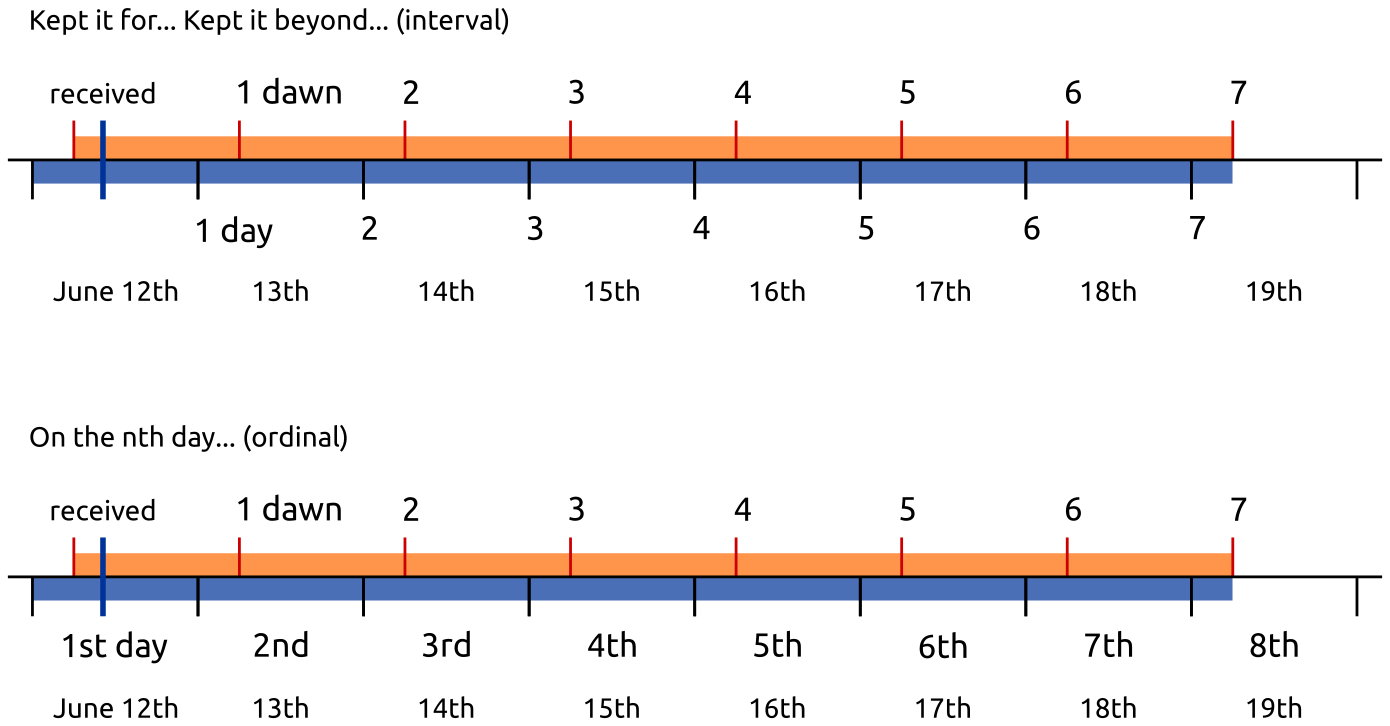
\includegraphics[width=\linewidth]{../../src/includes/figures/7-days.png}

\subsection{Breakfast tray}

After dawn, one receives a tray with bread, jams, honey, butter and
salt. At this point the lifetimes are:

\begin{itemize}
\tightlist
\item
  bread, jams: morning
\item
  honey, butter: 7 days
\item
  salt: lifetime
\end{itemize}

If the knife which one used carries bread morsels or jam into the honey
or the butter, these will be only allowable in the morning.

If one is careful to clean the knife and avoid mixing, one may use them
on the bread and keep the rest until their allowed lifetimes.

The next day, one receives a tray with only bread. One may \textbf{not}
mix the allowables from the previous day with the food received today.

Putting the salt, honey or butter (rec. yesterday) on the bread would be
Pc 38 (eating stored food).

\clearpage

\section{Pc 39, Requesting finer staple foods}

Finer staple foods: ghee, fresh butter, oil, honey, sugar, fish, meat,
milk, curds.

Object, effort, result.

Sk 37 covers non-fine staples: ``Not being ill, I will not eat rice or
bean curry that I have requested for my own sake: a training to be
observed.''

Hence, dukkata for requesting and consuming other staple foods, except
when one is ill.

\subsection{Non-offenses}

\emph{Not ill:} one is able to fare comfortably without these foods.

\begin{multicols}{2}

\begin{itemize}
\tightlist
\item
  being ill
\item
  was requested for the sake of an ill bhikkhu, and is now left over
\item
  from relatives
\item
  from those who gave invitation to ask
\item
  for the sake of another
\item
  from one's own resources
\end{itemize}

\end{multicols}

\section{Pc 47, Exceeding an invitation}

When an invitation is made that one may ask for certain requisites, one
may use it until four months, unless it has been repeated, or is a
permanent invitation.

\subsection{Non-offenses}

\begin{multicols}{2}

\begin{itemize}
\tightlist
\item
  from relatives
\item
  for the sake of another
\item
  from one's own resources
\item
  being ill, if one shows consideration
\end{itemize}

\end{multicols}

``The time period for which we were invited has passed, but we have need
of medicine.''

\section{Pc 41, Handing food to members of other religions}

One places oneself in the position of the followers of other religions.

It is not an offense to prepare food in a tray and placing it so that
they can help themselves.

\section{Pd 3, Protected families}

The purpose is to avoid damaging the faith of those supporters who might
suffer financially if they give too much.

\subsection{Non-offenses}

\begin{multicols}{2}

\begin{itemize}
\tightlist
\item
  being ill
\item
  invited
\item
  juice, tonics, medicines
\item
  the almsfood is supplied by others
\item
  the family members take turns
\item
  eating the leftovers of another bhikkhu
\item
  the family offers outside their residence
\end{itemize}

\end{multicols}


\chapter{Arguments 1}

\begin{itemize}
\tightlist
\item
  \textbf{Sg 10,} Schismatic group
\item
  \textbf{Sg 11,} Supporting a schismatic group
\item
  \textbf{Sg 12,} Not accepting admonishment
\item
  \textbf{Sg 13,} Not accepting a rebuke or banishment
\item
  \textbf{Pc 9,} Telling an unordained person about serious offence
\item
  \textbf{Pc 12,} Evasive reply
\item
  \textbf{Pc 13,} Criticising community official
\end{itemize}


\chapter{Dwellings}

\begin{itemize}
\tightlist
\item
  \textbf{Sg 6,} Too large hut without sponsor or approval
\item
  \textbf{Sg 7,} Large hut without approval
\item
  \textbf{Pc 14,} Leaving bed or bench
\item
  \textbf{Pc 15,} Spread bedding
\item
  \textbf{Pc 16,} Intruding on bhikkhu's sleeping place
\item
  \textbf{Pc 17,} Causing a bhikkhu to be evicted
\item
  \textbf{Pc 18,} Bed on an unplanked loft
\item
  \textbf{Pc 19,} Supervising the building work
\item
  \textbf{Pc 87,} Tall bed or bench
\item
  \textbf{Pc 88,} Cotton stuffing
\end{itemize}


\chapter{Arguments 2}

\begin{itemize}
\tightlist
\item
  \textbf{Pc 54,} Disrespectful after admonition
\item
  \textbf{Pc 64,} Concealing another's serious offence
\item
  \textbf{Pc 65,} Ordaining someone less than 20 years old
\item
  \textbf{Pc 68,} Not relinquishing an evil view
\item
  \textbf{Pc 69,} Suspended bhikkhu
\item
  \textbf{Pc 70,} Expelled novice
\item
  \textbf{Pc 74,} Hitting a bhikkhu
\item
  \textbf{Pc 75,} Threatening gesture
\end{itemize}


\chapter{Sekhiyas 1}

\begin{itemize}
\tightlist
\item
  \textbf{Sk 1-27,} Proper behaviour
\item
  \textbf{Sk 73-75,} Toilet etiquette
\end{itemize}


\chapter{Excuses}

\begin{itemize}
\tightlist
\item
  \textbf{Pc 71,} Ploy to avoid criticism
\item
  \textbf{Pc 72,} Criticising the rules
\item
  \textbf{Pc 73,} Claiming ignorance
\end{itemize}


\chapter{Food 3}

\begin{itemize}
\tightlist
\item
  \textbf{Pc 32,} Four bhikkhus specifically invited
\item
  \textbf{Pc 33,} Meal before invitation
\item
  \textbf{Pc 34,} More than three bowlfuls
\item
  \textbf{Pc 35,} More food after turning down what was offered
\item
  \textbf{Pc 36,} Tricking to break Pc 35
\end{itemize}


\chapter{Bowls}

\begin{itemize}
\tightlist
\item
  \textbf{NP 21,} Keeping extra bowl
\item
  \textbf{NP 22,} Asking for new bowl
\item
  \textbf{Pc 60,} Hiding another's requisites
\item
  \textbf{Pc 86,} Needle box
\end{itemize}


\chapter{Misc}

\begin{itemize}
\tightlist
\item
  \textbf{Pc 48,} Watching battle
\item
  \textbf{Pc 49,} Staying with army
\item
  \textbf{Pc 50,} Going to and army practice or review
\item
  \textbf{Pc 52,} Tickling
\item
  \textbf{Pc 53,} Playing in water
\item
  \textbf{Pc 55,} Attempting to frighten
\end{itemize}

\section{Pc 48, Watching battle}

\begin{multicols}{2}

Going to a battlefield to watch an army was a form of entertainment for
non-military citizens. Actual battle was not total warfare, and practice
manuveurs were outside the city.

Modern examples would include watching a public demonstration or a live
bradcast.

\textbf{Object:} an army on active duty. This is not only battle.

\textbf{Effort:} staying still and watching them is enough.

\textbf{Intention:} to watch them. Going to them for a different,
suitable reason is not an offense.

\columnbreak

\textbf{Non-offenses:}

\begin{itemize}
\tightlist
\item
  a suitable reason to go to the army (visiting an ill person, shelter
  from danger, invited for alms or to give a talk)
\item
  having other business, one sees the army
\item
  seeing them from the monastery
\item
  the army comes to where one happens to be
\item
  meeting an army coming from the opposite direction
\item
  there are dangers
\end{itemize}

\end{multicols}

\section{Pc 49, Staying with army}

If there is a suitable reason to go to an army, one may stay up to three
consecutive nights with the army.

The nights are counted as dawns.

\section{Pc 50, Going to and army practice or review}

While one is staying with an army, going to a battlefield (war games
included), roll call, the troops in battle formation or review.

Public parades, air shows are included.

Example: one visits the army for seeing a dying person. Later, in an
informal situation the soldiers are showing the monk how cool their
weapons are.

\section{Pc 52, Tickling}

A bhikkhu died from being unable to catch his breath while being
tickled.

\clearpage

\section{Pc 53, Playing in water}

\begin{multicols}{2}

\textbf{Effort:} one jumps up or down, splashes or swims.

\textbf{Object:} the water is at least ankle deep.

\emph{Dukkatas:} Paddling in a boat, sailing a sailboat or steering a
motorboat.

\textbf{Intention:} for fun, for a laugh.

Swimming for fitness is not mentioned, but there were monks known to
``keep their bodies in strong shape''. Ven. Dabba Mallaputta assigns
them to dwellings at the same place.

A medical instruction for swimming would be ``having business in the
water''.

\textbf{Non-offenses:}

\begin{itemize}
\tightlist
\item
  one has business to do in the water or in the boat
\item
  crossing to the other shore
\item
  there are dangers
\end{itemize}

\end{multicols}

\section{Pc 55, Attempting to frighten}

\textbf{Intention:} to frighten the other person.

\textbf{Effort:} any effort to make arrangements to cause fright, or
talking about dangers.

\textbf{Object:} the other person is a bhikkhu. \emph{Dukkata} for
non-bhikkhus.

Perception and Result are not factors.

\textbf{Non-offenses:} without the intention to cause fright.


\chapter{Sekhiyas 2}

\begin{itemize}
\tightlist
\item
  \textbf{Sk 27-56,} Food
\item
  \textbf{Sk 57-72,} Teaching Dhamma
\end{itemize}


\chapter{Robes 3}

\begin{itemize}
\tightlist
\item
  \textbf{NP 16,} Carrying Wool
\item
  \textbf{NP 26,} Thread
\item
  \textbf{NP 27,} Weavers
\item
  \textbf{NP 11-15,} Summary of santhatas
\end{itemize}


\chapter{Arguments 3}

\begin{itemize}
\tightlist
\item
  \textbf{Pc 77,} Provoking anxiety about a broken rule
\item
  \textbf{Pc 78,} Eavesdropping in an argument
\item
  \textbf{Pc 63,} Reopen a closed issue
\item
  \textbf{Pc 79,} Complaining about a community decision
\item
  \textbf{Pc 80,} Leaving a community meeting
\item
  \textbf{Pc 81,} Complaining about favouritism
\end{itemize}


\chapter{Misc}

\begin{itemize}
\tightlist
\item
  \textbf{Pc 4,} Teaching by rote
\item
  \textbf{Pc 5,} Lying down with unordained male
\item
  \textbf{Pc 42,} Sending a bhikkhu away
\item
  \textbf{Pc 43,} Intruding on an aroused couple
\item
  \textbf{Pc 83,} Entering a king's sleeping chamber unannounced
\item
  \textbf{As 1-7,} Summary of settling conflicts
\end{itemize}

\section{Pc 4, Teaching by rote}

\begin{multicols}{2}

Teaching a non-bhikkhu by reciting Dhamma with him line by line. That
is, training him to be skilled in recitation.

The offense includes novices.

The intention of the rule is guard the faith of lay people. If a teacher
makes mistakes, the student may lose respect for them. If the sessions
keep up for a time, the teacher might be seen as hired by the lay
person.

Dhamma here means Pali texts, and only those in the Pali Canon.

The definition doesn't include Mahayana sutras, translations and other
compositions.

\textbf{Non-offenses:}

\begin{itemize}
\tightlist
\item
  making someone recite in unison with another bhikkhu (student)
\item
  correcting or practicing a passage with a lay person which they are
  reading or already memorized (evening chanting)
\item
  a bhikkhu learning a passage from a lay person
\end{itemize}

\end{multicols}

\section{Pc 5, Lying down with unordained male}

\begin{multicols}{2}

Lying down in the same dwelling with an unordained male person for more
than three consecutive nights.

The intention of the rule is to avoid the lay people seeing the bhikkhus
in unsightly attitudes while sleeping.

\textbf{The same dwelling:} the interpretation is not fixed, as
dwellings come in many forms. Ideas used in various situations:

\begin{itemize}
\tightlist
\item
  the same roof
\item
  having a single common entrance
\item
  part of the same enclosure
\end{itemize}

Sometimes it may be the same building, other times the apartment, other
times the room.

\textbf{Three consecutive nights:} counted by dawns. If the bhikkhu or
the lay person gets up during the night, the count starts again.

The pacittiya is at lying down at the fourth night.

The lay person may be a different person from one night to the next, but
those nights are still consecutive.

\end{multicols}

\section{Pc 42, Sending a bhikkhu away}

\begin{multicols}{2}

Being together (on almsround or other business), sending the other
bhikkhu away with the intention to misbehave when being alone.

\textbf{Object:} another bhikkhu.

\textbf{Intention:} one wants to indulge in misconduct and does not want
him to see it.

Misconduct: laughing, playing, sitting in private with a woman, etc.

\textbf{Effort:} one dismisses him, sending him away by direct command
or indirect remarks

\textbf{Result:} he leaves one's range of hearing and sight.

\textbf{Non-offenses:} dismissing him for a different reason.

\end{multicols}

\section{Pc 43, Intruding on an aroused couple}

\begin{multicols}{2}

Entering or staying in the same private part (bedroom) of the dwelling
where at least one of the couple is aroused for intercourse.

\textbf{Object:} the aroused couple.

\textbf{Effort:} sitting in the same private part of the dwelling
without another bhikkhu present.

Perception is not a factor. Better ask to make sure one is welcome to
stay.

\textbf{Non-offenses:}

\begin{itemize}
\tightlist
\item
  both the man and woman have left the private area
\item
  neither of them is aroused
\item
  the building is not for sleeping
\item
  the bhikkhu is not in the private area
\item
  another bhikkhu is present
\end{itemize}

\end{multicols}

\section{Pc 83, Entering a king's sleeping chamber unannounced}

\begin{multicols}{2}

Entering the sleeping chamber without announcement one might suprise the
couple in an intimate situation.

The situation is relevant when one is on familiar terms with any person
of influence. Annoying him, being in a suspicous situation, or meeting
enticing circumstances can be dangerous for the bhikkhu.

\end{multicols}

\section{As 1-7, Summary of settling conflicts}

Adhikaraṇa-samatha, `the settling of issues'. Procedures for settling:
a) disputes, b) accusations, c) offenses, d) duties.

\subsection{1. A face-to-face verdict should be given.}

The community must be qualified to carry out the transaction. The
individuals involved in the matter must be present. The principles of
Dhamma-Vinaya must be the guides for the group.

\subsection{2. A verdict of mindfulness may be given.}

Verdict of innocence, based on that the accused remembers fully that he
did not commit the offense.

\subsection{3. A verdict of past insanity may be given.}

Verdict of innocence, based on that the accused was out of his mind when
he committed the offense and so is absolved of any resposibility for it.

\clearpage

\subsection{4. Acting in accordance with what is admitted.}

\textbf{A)} Ordinary confession with no formal interrogation.

\textbf{B)} Following an accusation the community interrogates the
bhikkhu, he admits doing the action, and the community proceeds
according the severity of the offense.

\subsection{5. Acting in accordance with the majority.}

In cases when there is no unanimous agreement among the bhikkhus the
decision can be made by majority vote.

\subsection{6. Acting for his further punishment.}

The bhikkhu drags out an issue and only admits to the offense after a
formal interrogation. A further punishment must be imposed on the
bhikkhu for being so uncooperative.

\subsection{7. Covering over as with grass.}

Both sides realize that they are unable to resolve the dispute and
further meetings will only result in greater divisiveness. If both sides
agree, they gather in one place with every bhikkhu in the territory
present (no one should send his consent). A representative of each side
addresses the entire group and makes the blanket confession.



\backmatter

\chapter{Profiles}

\section{Ven. Anuruddha}

\href{https://what-buddha-said.net/library/DPPN/ay/anuruddha.htm}{DPPN,
Anuruddha}

\section{Chabbaggiya, the group of six}

\href{https://what-buddha-said.net/library/DPPN/c/chabbaggiyaa.htm}{DPPN,
Chabbaggiya}

\href{https://what-buddha-said.net/library/ati_website/html/lib/authors/hecker/wheel263.html}{Wheel
263}

\section{Ven. Udāyin}

\href{https://what-buddha-said.net/library/DPPN/u/udaayii.htm}{DPPN,
Udāyī}

\href{https://what-buddha-said.net/library/DPPN/l/laludayi_th.htm}{DPPN,
Lāludāyī Thera}



\chapter{Questions}

\section{Introduction}

How can the monks determine if a modern item (e.g.~credit cards, sun
glasses) are allowable or not?

How does one determine whether there is full offence of a rule?

Could the abbot of a small monastery ordain a \emph{bhikkhu} or
\emph{samanera}? What should he do?

Advice on restoring one's faith after breaking a rule or having done
something unbecoming.

\section{Killing and harming}

The loved family dog of a lay supporter is very ill, and treatment will
be expensive. He asks a monk whether they should ask the vet to
euthanise the dog, or apply for treatment.

A woman asks a monk if she should get an abortion. What should the monk
say?

A monk discovers a tick on his arm. What should he do?

A monk hits an anagarika. What should the anagarika do?

\section{Stealing}

A monk sneaks into the kitchen and eats an apple. Did he steal it?

A lay supporter brings an expensive sweet and gives it to a monk, saying
`I brought this for the abbot'. The monk eats a bit from it before
giving it to the abbot. Did he steal it?

A monk is visiting a monastery and makes a long phone call. The call
costs 100 EUR. The resident monks discover it on the bill and ask if
anyone knows about this call. He remains silent.

How is it possible for a monk to steal from the Sangha?

A monk drives away with the monastery car and never comes back.
Consequences?

\section{Lustful conduct}

A monk curses with lewd words in front of a woman.

A married couple wants to ask a monk how to live together peacefully.

A monk is carrying a table with a woman and he playfully pushes it into
her.

A monk receives treatment on his tooth from a female dentist.

A monk is trying on shoes in a shop. A female assistant helps to put on
a shoe and she asks, ``Is that comfortable?''

\section{Women 1}

\enlargethispage{2\baselineskip}

A monk is travelling by train, sitting in a compartment alone. At one of
the stops a woman enters and takes a seat in the compartment.

A monk stays at his parents' house for a night.

A monk is travelling by bus to visit a friend. He arrives at the bus
station, and the girlfriend of his friend is there with a car to pick
him up. She asks the monk to call his friend and tell him she will be
back at their apartment shortly.



\end{document}

